\documentclass[9pt]{beamer}


%\usepackage{bibunits}
 %\addbibresource{literature.bib}
% \usepackage{algorithm,algorithmic}
\usepackage{amsmath}
% \usepackage{stmaryrd}
% \usepackage{longtable}
% \usepackage{proof,mathpartir}
% \usepackage{fix-cm}
% \usepackage{bm}
% \usepackage{listings}
% \usepackage{amssymb}
% \usepackage{colortbl}
 \usepackage{tcolorbox}
% \usepackage{dsfont}
% \usepackage{amsfonts}
% \usepackage{ulem,xcolor}
% \usepackage{xspace}
% \usepackage{eqparbox}
% \usepackage{siunitx,amsmath}
\definecolor{safetyred}{RGB}{200,0,0}
\definecolor{traceblue}{RGB}{0,80,200}
\definecolor{codegray}{rgb}{0.95,0.95,0.95}
\definecolor{commentgreen}{rgb}{0.0,0.5,0.0}
\definecolor{keywordblue}{rgb}{0.0,0.0,0.8}
\definecolor{alertred}{rgb}{0.8,0.0,0.0}
\input{macrossl.tex}

% % Code Listing Settings
% \lstset{
%   backgroundcolor=\color{codegray},
%   commentstyle=\color{commentgreen},
%   keywordstyle=\color{keywordblue}\bfseries,
%   basicstyle=\ttfamily\small,
%   breaklines=true,
%   columns=fullflexible,
%   frame=single,
%   showstringspaces=false,
%   captionpos=b,
%   tabsize=2
% }
% \lstdefinelanguage{YAML}{
%   keywords={true, false, null, y, n},
%   keywordstyle=\color{darkgray}\bfseries,
%   basicstyle=\ttfamily\footnotesize,
%   commentstyle=\color{teal}\itshape,
%   stringstyle=\color{blue},
%   morestring=[b]',
%   morestring=[b]",
%   morecomment=[l]{\#},
%   moredelim=[l][\color{orange}]{\&},
%   moredelim=[l][\color{magenta}]{*},
%   moredelim=**[il][\color{red}]{:},
%   literate={---}{{\textcolor{gray}{---}}}3
% }

%\addbibresource{literature.bib}
% \newcommand\mCite[1]{[\cite{#1}, \citetitle{#1}]}
% \newcommand{\itemEq}[1]{%
% 	\begingroup%
% 	\setlength{\abovedisplayskip}{0pt}%
% 	\setlength{\belowdisplayskip}{0pt}%
% 	\parbox[c]{\linewidth}{\begin{flalign}#1&&\end{flalign}}%
% 	\endgroup}
% \renewcommand\algorithmiccomment[1]{%
% 	\hfill\#\ \eqparbox{COMMENT}{#1}%
% }



% Encoding
\usepackage[T1]{fontenc}
% UTF8 input
\usepackage[utf8]{inputenc}
% Use german language
\usepackage[english]{babel}
\renewcommand{\arraystretch}{1.3}

% Use the given theme
\usetheme{HLISP}
%\renewcommand{\algorithmicforall}{\textbf{foreach}}
\title{Formal Modeling and Analysis of Metric-Timed Systems and Multi-Agent Normative Specifications of Actions}
% \subtitle{\footnotesize\textbf{Supervisor:}\\ Prof. Dr. Martin Leucker \\
% \textbf{Second Referee:}\\ Prof. Dr. Gordon J. Pace \\
%   \textbf{Chair of the Examination Committee:}\\ Prof. Dr. Stefan Fischer}

\author{
  PhD Candidate: Karam Younes Kharraz
}
\date{29 April 2026}

\begin{document}

% --- Title ---
\begin{frame}
  \titlepage
\end{frame}

\begin{frame}{Outline}
	\tableofcontents
  \end{frame}
\section{Introduction and Context}
\begin{frame}{The Cost of Normative Compliance}
  \begin{columns}
    \begin{column}{0.5\textwidth}
      \textbf{Motivation:}
      \begin{itemize}
        \item Normative systems govern behavior via \textbf{ought-to-do rules}.
        \item Manual verification creates a heavy economic burden.
        \item Real-world rules involve strict \textbf{time constraints} and \textbf{distributed agents}.
      \end{itemize}
      
      \vspace{0.3cm}
      \textbf{The Problem:}
      \begin{itemize}
        \item Fragments of laws often \textbf{conflict} (ambiguity).
        \item Accountability fails when multi-agent collaboration breaks down.
      \end{itemize}
    \end{column}

    \begin{column}{0.5\textwidth}
      \centering
      \begin{tikzpicture}[scale=0.8, transform shape, node distance=1.8cm]
        % Manual Process
        \node (rulebook) [rectangle, draw, thick, minimum width=2.5cm, minimum height=1.2cm, align=center, fill=gray!10] {Manual\\Rulebook};
        \node (maze) [rectangle, draw, thick, below of=rulebook, minimum width=2.5cm, minimum height=1.2cm, align=center, fill=red!20] {Administrative\\Bottleneck};
        \draw [->, thick] (rulebook) -- (maze);

        % Digital Process
        \node (digital) [rectangle, draw, thick, right=2cm of rulebook, minimum width=2.5cm, minimum height=1.2cm, align=center, fill=blue!10] {Formal\\Rules};
        \node (flow) [rectangle, draw, thick, below of=digital, minimum width=2.5cm, minimum height=1.2cm, align=center, fill=green!20] {Automated\\Compliance};
        \draw [->, thick] (digital) -- (flow);

        \draw [dashed, thick, gray] (1.25,-0.6) -- (1.25,-2.8);
      \end{tikzpicture}
    \end{column}
  \end{columns}
\end{frame}

\begin{frame}{Research Directions}
  \begin{tcolorbox}[colback=blue!5, colframe=blue!80, title=RD1 / Chapter 2: Static Conflict Analysis]
    How can we formally detect, measure, and explain conflicts between time-constrained obligations and prohibitions?
  \end{tcolorbox}
  
  



  
  \begin{tcolorbox}[colback=green!5, colframe=green!80, title=RD2 / Chapter 3: Blame Attribution in multi-agent setting]
    How do we formalize and quantify responsibility when collaborative execution of norms fails in a multi-agent setting?
  \end{tcolorbox}
\end{frame} 





\begin{frame}{Methodology: Micro Metric-Time Normative Logic ($\TDDLfm$)}
  \begin{block}{Syntax: restricted to essential structures for practitioners}
    Focus on precisely timed \textbf{Obligations} ($O$) and \textbf{Prohibitions} ($F$).
    \[
    \phi ::= \ob{\is}{a} \mid \forb{\is}{a} \mid \phi \sqcap \phi \mid \phi \sqcup \phi
    \]
    Where $\mathfrak{I}$ is a canonical set of disjoint time intervals.
  \end{block}

  \begin{block}{The Analysis Pipeline: From sat to conflict characterisation and repair}
\begin{enumerate}
  \item Sat resolution: Determine if a specification is satisfiable.
  \item Conflict static definition: Deontic and Ontic conflicts.
  \item Conflict measurement: Quantify the degree of conflict using a novel metric.
  \item Conflict characterization: If not fully conflicting, eliminate the minimal unsatisfiable subsets (MUSes) to explain the conflict.
\end{enumerate}
  \end{block}
\end{frame}

\begin{frame}{Discussion: Visualizing Conflict Resolution}
  \centering
  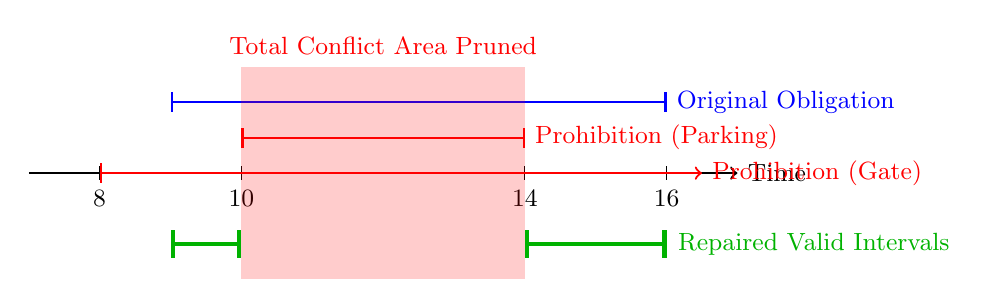
\begin{tikzpicture}[scale=0.9, every node/.style={font=\small}]
    % Time axis
    \draw[->, thick] (7,0) -- (17,0) node[right] {Time};
    \foreach \x in {8, 10, 14, 16} \draw (\x,0.1) -- (\x,-0.1) node[below] {\x};

    % Original Contract
    \draw[blue, thick, |-|, yshift=1cm] (9,0) -- (16,0) node[right] {Original Obligation};
    
    % Prohibition 1
    \draw[red, thick, |-|, yshift=0.5cm] (10,0) -- (14,0) node[right] {Prohibition (Parking)};
    
    % Prohibition 2
    \draw[red, thick, |->, yshift=0cm] (8,0) -- (16.5,0) node[right] {Prohibition (Gate)};
    
    % Repaired
    \draw[green!70!black, ultra thick, |-|, yshift=-1cm] (9,0) -- (10,0);
    \draw[green!70!black, ultra thick, |-|, yshift=-1cm] (14,0) -- (16,0) node[right] {Repaired Valid Intervals};

    % Highlight conflict zone
    \fill[red, opacity=0.2] (10,-1.5) rectangle (14, 1.5);
    \node at (12, 1.8) {\textcolor{red}{Total Conflict Area Pruned}};
  \end{tikzpicture}
\end{frame}



\begin{frame}{Key Results: The Blame Attribution Procedure}
  \begin{itemize}
    \item Formalized \textbf{Obligation task of an agent as}: \textit{"Agent $x$ has to accomplish task $a$ ..."}
    \item Quantified blame based on the lack of \textit{attempt} over a defined duration.
  \end{itemize}

  \vspace{0.5cm}
  \centering
  \begin{tikzpicture}[scale=0.9]
    \node (trace) [rectangle, draw, thick, minimum width=2cm, align=center, fill=gray!10] {Execution Trace Monitoring};
    
    \node (sat) [rectangle, draw=green, thick, fill=green!10, below left=1cm and 1cm of trace, align=center] {\textbf{Satisfied}\\Both attempted};
    \node (part) [rectangle, draw=orange, thick, fill=orange!10, below=1cm of trace, align=center] {\textbf{Partial Failure}\\One agent lacks attempt};
    \node (viol) [rectangle, draw=red, thick, fill=red!10, below right=1cm and 1cm of trace, align=center] {\textbf{Violated}\\Both failed attempt};
    
    \draw[->, thick] (trace) -- (sat);
    \draw[->, thick] (trace) -- (part);
    \draw[->, thick] (trace) -- (viol);
    
    \draw[->, thick, dashed, orange] (part) |- ++(0,-1.5) -| node[pos=0.25, below, font=\small] {Calculates responsibility ratio} (viol);
  \end{tikzpicture}
\end{frame}



\begin{frame}{Conclusion}
  \begin{tcolorbox}[colback=uzlmain!5, colframe=uzlmain, title=Core Takeaway]
    Restricting logical expressivity in a principled manner enables stronger, operational forms of automated reasoning about normative systems.
  \end{tcolorbox}
  
  \vspace{0.4cm}
  
  \textbf{Summary of Deliverables:}
  \begin{enumerate}
    \item \textbf{$\mathsf{MTNL}$}: Formal pipeline for timed conflict detection.
    \item \textbf{Automated Repair}: Algorithms balancing conciseness and conflict elimination.
    \item \textbf{$\mathsf{cDL}$}: Deepened dynamic analysis via blame attribution in multi-agent task collaboration and in a perpetual manner.
  \end{enumerate}
\end{frame}

\begin{frame}{Future Work}
  \begin{block}{Toward a Unified Formalism ($\mathsf{MTTACNL}$)}
    Mixing the timed $\TDDLfm$ with  the multi-agent aspect of $\cDL$ and getting both conflict and monitoring algoirthms for this setting.
  \end{block}

  \begin{itemize}
    \item \textbf{ITP integration} Integrating the logics into interactive theorem provers (e.g., Roq, Lean).
    \item \textbf{Moving beyond Discrete actions:} Actions with directions and continous states(ought-to-be).
  \end{itemize}
\end{frame}
	
	
	
\end{document}